%
\documentclass[%
 reprint,
 amsmath,amssymb,
 aps,
]{revtex4-1}

\usepackage{graphicx}% Include figure files
\usepackage{dcolumn}% Align table columns on decimal point
\usepackage{bm}% bold math


\begin{document}
\title{Caratula}

\begin{titlepage}
\begin{center}
\large{UNIVERSIDAD PRIVADA DE TACNA}\\
\vspace*{-0.025in}
\begin{figure}[htb]
\begin{center}

\includegraphics[width=8cm]{./Imagenes/logo}
\end{center}
\end{figure}
\vspace*{0.15in}
INGENIERIA DE SISTEMAS  \\

\vspace*{0.5in}
\begin{large}
TITULO:\\
\end{large}

\vspace*{0.1in}
\begin{Large}
\textbf{Trabajo-Encargado-N-05-SQL-y-NoSQL} \\
\end{Large}

\vspace*{0.3in}
\begin{Large}
\textbf{CURSO:} \\
\end{Large}

\vspace*{0.1in}
\begin{large}
BASE DE DATOS II\\
\end{large}

\vspace*{0.3in}
\begin{Large}
\textbf{DOCENTE(ING):} \\
\end{Large}

\vspace*{0.1in}
\begin{large}
 Patrick Cuadros Quiroga\\
\end{large}

\vspace*{0.2in}
\vspace*{0.1in}
\begin{large}
Integrantes: \\
\begin{flushleft}
Adnner Esperilla Ruiz		\hfill	(2015050543) \\
Wilfredo Vilca Chambilla		\hfill	(2006028540) \\

\vspace*{0.5in}
\begin{center}
2019-Tacna\\
\end{center}
\vspace*{2in}
\end{flushleft}
\end{large}
\end{center}

\end{titlepage}



\title{SQL vs NoSQL}


\begin{abstract}
\begin{center}
\vspace*{0.5in}
\textbf{Resumen}
\end{center}

En este artículo aprenderemos conceptos ,metodos y usos sobre las base de datos SQL y NOSQL, y tambien sus diferencias entre ellos. Esto nos permitirá elegir cuall es la mejor la opción más recomendable para nuestro uso ,ya que cuando se da un proyecto se genera la dudo de que gestor de base de datos nos conviene usar .\\


\begin{center}

\end{center}


\end{abstract}


\maketitle

%\tableofcontents

\section {Introducción}\label{sec:1}
Las tecnologías NoSQL han evolucionado para dar respuesta a distintos problemas, y aunque tienen muchos aspectos en común, también son muy diferentes entre sí. Dada la diversidad de tecnologías NoSQL, habitualmente se clasifican en cuatro grupos, por su forma de modelar los dato.
Son muchas las aplicaciones web que utilizan algún tipo de bases de datos para funcionar. Hasta ahora estábamos acostumbrados a utilizar bases de datos SQL como son MySQL pero desde hace ya algún tiempo han aparecido otras que reciben el nombre de NoSQL  y que han llegado con la intención de hacer frente a las bases relacionales utilizadas por la mayoría de los usuarios.



%-----------------------------------------------------------------
\section{Objetivos}\label{sec:2}
\subsection{General:}
-  Poder distinguir las principales caracteristicas  entre  SQL y  NoSQL.
\subsection{Específicos:}
-  Comparar el concepto de bases de datos SQL Y  NoSQL, además de presentar sus ventajas y compararlos con otros sistemas de bases de datos.


%-----------------------------------------------------------------
\section {Marco Teórico}\label{sec:3}
\subsection{BASE DE DATOS}
\par Una base de datos es un conjunto de datos pertenecientes a un mismo contexto y almacenados sistemáticamente para su posterior uso. En este sentido; una biblioteca puede considerarse una base de datos compuesta en su mayoría por documentos y textos impresos en papel e indexados para su consulta. Actualmente, y debido al desarrollo tecnológico de campos como la informática y la electrónica, la mayoría de las bases de datos están en formato digital, siendo este un componente electrónico, por tanto se ha desarrollado y se ofrece un amplio rango de soluciones al problema del almacenamiento de datos.Coniene las siguientes caracteristicas:
\begin{itemize}
	\item Se emplean métodos determinados para incluir datos nuevos y para borrar, modificar o recuperar los datos almacenados.
	\item Los datos son independientes de los programas que los usan.
	\item Los datos están interrelacionados, sin redundancias innecesarias.
\end{itemize}
\subsection {SISTEMA DE GESTIÓN DE BASE DE DATOS}
Un sistema gestor de base de datos (SGBD) es un conjunto de programas que permiten el almacenamiento, modificación y extracción de la información en una base de datos .Los usuarios pueden acceder a la información usando herramientas específicas de consulta y de generación de informes, o bien mediante aplicaciones al efecto.
Generalmente se accede a los datos mediante lenguajes de consulta, lenguajes de alto nivel que simplifican la tarea de construir las aplicaciones. También simplifican las consultas y la presentación de la información. Un SGBD permite controlar el acceso a los datos, asegurar su integridad, gestionar el acceso concurrente a ellos, recuperar los datos tras un fallo del sistema y hacer copias de seguridad. Las bases de datos y los sistemas para su gestión son esenciales para cualquier área de negocio, y deben ser gestionados con esmero.
Es una aplicación comercial que permite construir y gestionar bases de datos, proporcionando al usuario de la Base de Datos las herramientas necesarias para realizar, al menos, las siguientes tareas:
\begin{itemize}
	\item Mantener la integridad de la información.
	\item Proporcionar control de la privacidad y seguridad de los datos en la Base de Datos, permitiendo sólo el acceso a los mismos a los usuarios autorizados.
	\item Definir las estructuras de los datos.
	\item Manipular los datos. Es decir, insertar nuevos datos, así como modificar, borrary consultar los datos existentes.
\end{itemize}

\subsection{ Structured Query Language}
\par El lenguaje estructurado de consultas (SQL, Structured Query Language) apoya la creación y mantenimiento de la base de datos relacional y la gestión de los datos dentro de la base de datos. (Fundamentos SQL)

El modelo relacional, el cual se basa principalmente en los principios matemáticos de la teoría de conjuntos y lógica de predicados, apoya la recuperación de datos sencilla, aplica la integración de datos (la precisión y coherencia de los datos), y proporciona una estructura de base de datos independiente de las aplicaciones al acceder a los datos almacenados.
El modelo relacional tiene como estructura de almacenamiento de los datos las relaciones. La intensión o esquema de una relación consiste en el nombre que hemos dado a la relación y un conjunto de atributos. La extensión de una relación es un conjunto de tuplas. Al trabajar con SQL, esta nomenclatura cambia, como podemos apreciar en la siguiente figura:
\begin{figure}[htb]
	\begin{center}
	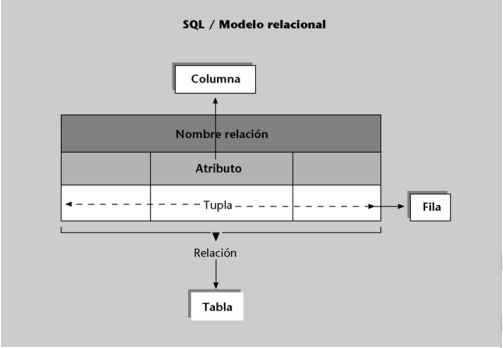
\includegraphics[width=7cm]{./Imagenes/SQLmodelo.png}
	\end{center}
	\end{figure}
\par Ejemplo:
\begin{figure}[htb]
	\begin{center}
	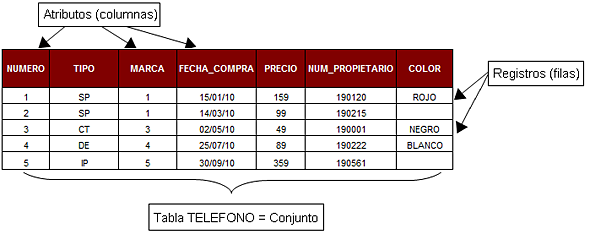
\includegraphics[width=7cm]{./Imagenes/SQLmodelo2.png}
	\end{center}
	\end{figure}
\par Una máquina virtual es un software que emula un ordenador justo como si fuese uno real. Todo esto sucede en una ventana dentro de tu sistema operativo actual como cualquier otro programa que uses.
\par Cómo funciona:
	\begin{itemize}
		\item Cuando creas una máquina virtual para instalar otro sistema operativo tendrás que asignar todos los recursos que necesitas.
	\end{itemize}

   \par VENTAJAS:
\\
\begin{itemize}
		\item Alta velocidad; las consultas SQL pueden utilizarse para recuperar grandes cantidades de registros de una base de datos de forma rápida y eficiente.
		\item No necesita codificación; el uso de SQL estándar es más fácil administrar sistemas de bases de datos sin tener que escribir una cantidad sustancial de código.
		\item Estándares bien definidos
		\item Portablilidad
		\item Lenguaje interactivo
		\item Vista de datos múltiples
	\end{itemize}

   \par DESVENTAJAS:
\\                
\begin{itemize}
		\item Dificultad en la interfaz; la interconexión de una base de datos SQL es mas compleja que agregar algunas líneas de código.
		\item Más funciones implementadas de forma patentada; algunas bases de datos se dirigen a 
extensiones propietarias a SQL estándar para garantizar el bloqueo del proveedor.
	\end{itemize}


\subsection{NoSQL}
\par NoSQL aparece con la llegada de la web 2.0 ya que hasta ese momento sólo subían contenido a la red aquellas empresas que tenían un portal, pero con la llegada de aplicaciones como Facebook, Twitter o Youtube, cualquier usuario podía subir contenido, provocando así un crecimiento exponencial de los datos.

\par Es en este momento cuando empiezan a aparecer los primeros problemas de la gestión de toda esa información almacenada en bases de datos relacionales. En un principio, para solucionar estos problemas de accesibilidad, las empresas optaron por utilizar un mayor número de máquinas pero pronto se dieron cuenta de que esto no solucionaba el problema, además de ser una solución muy cara. La otra solución era la creación de sistemas pensados para un uso específico que con el paso del tiempo han dado lugar a soluciones robustas, apareciendo así el movimiento NoSQL. 
\par Además de lo comentado anteriormente, las bases de datos NoSQL son sistemas de almacenamiento de información que no cumplen con el esquema entidad–relación. Tampoco utilizan una estructura de datos en forma de tabla donde se van almacenando los datos sino que para el almacenamiento hacen uso de otros formatos como clave–valor, mapeo de columnas o grafos.


\par Beneficios:
	Esta forma de almacenar la información ofrece ciertas ventajas sobre los modelos relacionales. Entre las ventajas más significativas podemos destacar:
	\begin{itemize}
		\item Se ejecutan en máquinas con pocos recursos: Estos sistemas, a diferencia de los sistemas basados en SQL, no requieren de apenas computación, por lo que se pueden montar en máquinas de un coste más reducido.
		\item Escalabilidad horizontal: Para mejorar el rendimiento de estos sistemas simplemente se consigue añadiendo más nodos, con la única operación de indicar al sistema cuáles son los nodos que están disponibles.
		\item Pueden manejar gran cantidad de datos: Esto es debido a que utiliza una estructura distribuida, en muchos casos mediante tablas Hash.(asocia llaves o claves con valores).\cite{hash}
		\item No genera cuellos de botella: El principal problema de los sistemas SQL es que necesitan transcribir cada sentencia para poder ser ejecutada, y cada sentencia compleja requiere además de un nivel de ejecución aún más complejo, lo que constituye un punto de entrada en común, que ante muchas peticiones puede ralentizar el sistema. \cite{acens}
	\end{itemize}
	\begin{figure}[htb]
	\begin{center}
	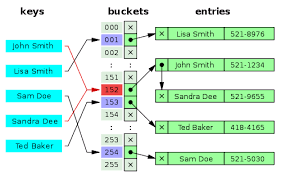
\includegraphics[width=7cm]{./Imagenes/hash}
	\end{center}
	\end{figure}

           \par TIPOS PARA ALMACENAR INFORMACIÓN EN BASE DE DATOS NOSQL
\\        
\\  
  -  Base de Datos Orientadas a Documentos:
\\
           \begin{figure}[htb]
	\begin{center}
	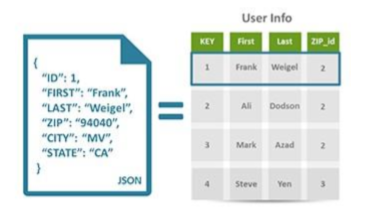
\includegraphics[width=7cm]{./Imagenes/1}
	\end{center}
	\end{figure}
\\
 Este tipo almacena la información como un documento, generalmente utilizando para ello una estructura simple como JSON o XML y donde se utiliza una clave única para cada registro. Este tipo de implementación permite, además de realizar búsquedas por clave–valor, realizar consultas más avanzadas sobre el contenido del documento.  
Son las bases de datos NoSQL más versátiles. Se pueden utilizar en gran cantidad de proyectos, incluyendo muchos que tradicionalmente funcionarían sobre bases de datos relacionales. \cite{TiposNoSQL}
Algunos ejemplos de este tipo son:
           \begin{itemize}
		\item MongoDB
		\item CouchDB
		\item RaveDB
		\item SimpleDB (Amazon)
	\end{itemize}

 -  Base de datos key-value:
\\
\\

	\begin{center}
	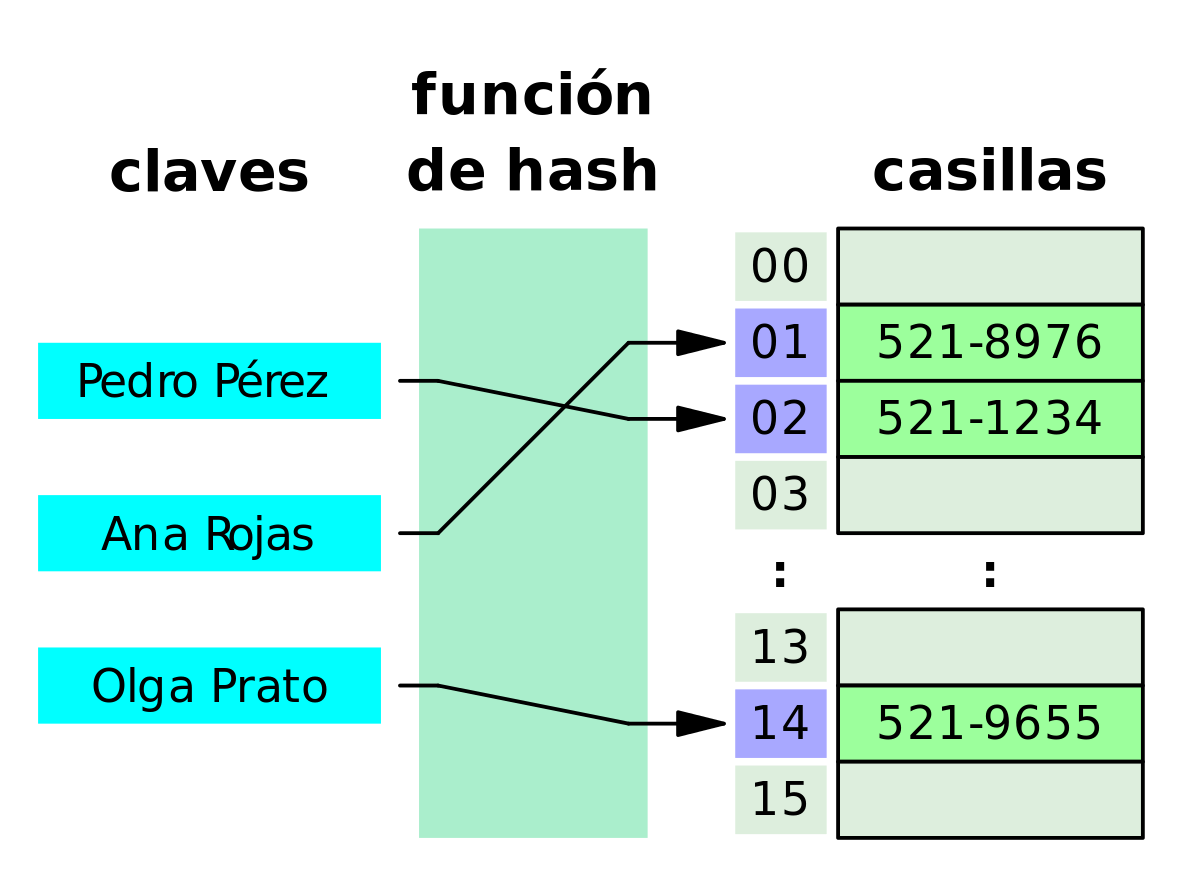
\includegraphics[width=7cm]{./Imagenes/2}
	\end{center}
Son el modelo de base de datos NoSQL más popular, además de ser la más sencilla en cuanto a funcionalidad. En este tipo de sistema, cada elemento está identificado por una llave única, lo que permite la recuperación de la información de forma muy rápida, información que habitualmente está almacenada como un objeto binario (BLOB). Se caracterizan por ser muy eficientes tanto para las lecturas como para las escrituras.  \cite{acens}
Algunos ejemplos de este tipo son :
           \begin{itemize}
		\item Cassandra (Apache)
		\item Riak
		\item Redis
		\item Dynamo (Amazon)
                     \item Dynamo (Amazon)
                     \item BigTable (Google)
	\end{itemize}
-  Base de datos en grafo:
\\
\\

	\begin{center}
	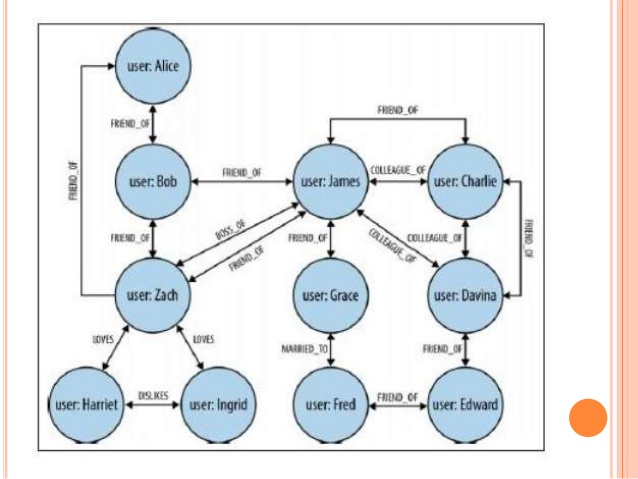
\includegraphics[width=7cm]{./Imagenes/3}
	\end{center}
En este tipo de bases de datos, la información se representa como nodos de un grafo y sus relaciones con las aristas del mismo, de manera que se puede hacer uso de la teoría de grafos para recorrerla. Para sacar el máximo rendimiento a este tipo de bases de datos, su estructura debe estar totalmente normalizada, de forma que cada tabla tenga una sola columna y cada relación dos. 
Este tipo de bases de datos ofrece una navegación más eficiente entre relaciones que en un modelo relacional. \cite{acens}
Algunos ejemplos de este tipo son:
           \begin{itemize}
		\item Neo4j
		\item Dex
		\item Sones GraphBD
		\item AllegroGraph
	\end{itemize}
-  Base de datos orientadas a objetos:
\\
\\
En este tipo, la información se representa mediante objetos, de la misma forma que son representados en los lenguajes de programación orientada a objetos (POO) como ocurre en JAVA, Cchar o Visual Basic .NET. \cite{acens}
Algunos ejemplos de este tipo de bases de datos son : 

           \begin{itemize}
		\item ObjectDB
		\item ZooDB
		\item DB4o
	\end{itemize}

- Nosql es "más adecuado" en estos escenarios por lo menos:
   \begin{itemize}
		\item Fácil de escalar simplemente agregando más nodos.
		\item Consulta sobre conjunto de datos de gran tamaño.En RDMS, podría haber tablas con millones (¿o miles de millones?) De filas, y no desea hacer consultas en esas tablas directamente, ni siquiera mencionar, la mayoría de las veces, las combinaciones de tablas también son necesarias para consultas complejas.
		\item Cuello de botella en la E / S del disco Si un sitio web necesita enviar resultados a diferentes usuarios en función de la información en tiempo real de los usuarios, probablemente estamos hablando de decenas o cientos de miles de solicitudes de lectura / escritura de SQL por segundo\cite{No}
	\end{itemize}
- EJEMPLO:
Los métodos insertOne(<document>) e insertMany([<doc1>,<doc2>…]) implícitamente crean una collection si no existe e insertan uno o muchos documents según sea el caso. Por si no se dieron cuenta en Mongo no tuvimos que especificar el “id” de nuestro document, si no definimos un campo “id”, Mongo lo crea automáticamente.El método updateMany(<filter>,<update>) actualiza múltiples documents dentro de una collection basado en el filtro que recibe como argumento, pero además puede alterar los documents con operaciones de set (establecer) y unset (des-establecer) para agregar o borrar fields. Como vemos la forma de alterar información en Mongo no se hace a nivel de collections ya que no es una modificación estructural sino de documents (registros de nuestra colección).Con insert nosotros podemos agregar registros a nuestra definición de datos. En Mongo ya vimos la forma de hacer estos inserts con los métodos insertOne() e insertMany().\cite{NoSQL}

	\begin{center}
	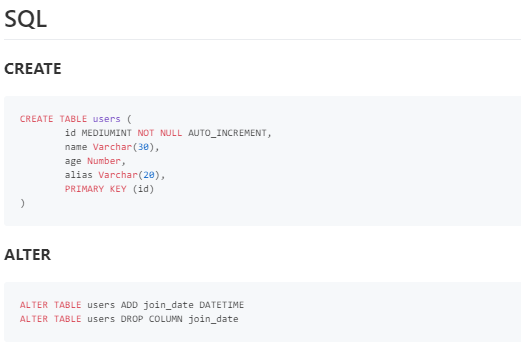
\includegraphics[width=7cm]{./Imagenes/4}
          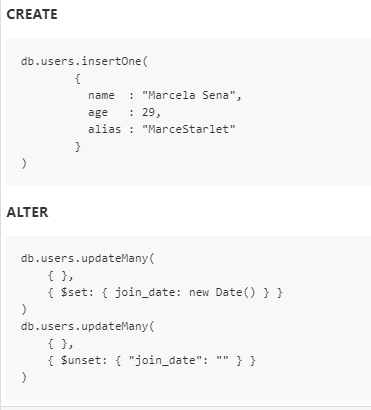
\includegraphics[width=7cm]{./Imagenes/5}
	\end{center}
\subsection{SQL vs NoSQL}

	\begin{center}
	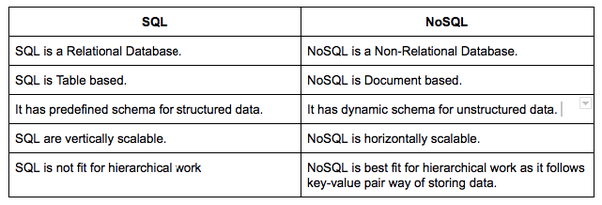
\includegraphics[width=7cm]{./Imagenes/tablasqlno}
	\end{center}
	\par NoSQL: 
	\begin{itemize}
	\item No utilizan estructuras fijas como tablas para el almacenamiento de los datos. Permiten hacer uso de otros tipos de modelos de almacenamiento de información como sistemas de clave–valor, objetos o grafos.
	\item No suelen permitir operaciones JOIN. Al disponer de un volumen de datos tan extremadamente grande suele resultar deseable evitar los JOIN. Esto se debe a que, cuando la operación no es la búsqueda de una clave, la sobrecarga puede llegar a ser muy costosa. Las soluciones más directas consisten en desnormalizar los datos, o bien realizar el JOIN mediante software, en la capa de aplicación.
	\item Arquitectura distribuida. Las bases de datos relacionales suelen estar centralizadas en una única máquina o bien en una estructura máster–esclavo, sin embargo en los casos NoSQL la información puede estar compartida en varias máquinas mediante mecanismos de tablas Hash distribuidas.
	\end{itemize}
	\cite{comparison}
	

%-----------------------------------------------------------------
\section{Conclusiones}\label{sec:6}


\begin{itemize}
	\item La selección de la tecnología de almacenamiento adecuada involucra la consideración de numerosos aspectos. Aunque el rendimiento suele ser el factor más importante, es necesario considerar aspectos como la funcionalidad, la facilidad de operación, sencillez de uso, disponibilidad de profesionales con conocimiento, seguridad, y otros factores como la existencia de herramientas y una comunidad que respalde el producto. independiente.
	\item Cada vez con más frecuencia estamos viendo cómo las tecnologías NoSQL forman parte de la solución en proyectos empresariales, gracias a beneficios como la mejora en la productividad de los equipos de desarrollo, y la posibilidad de llegar antes al mercado y con una considerable reducción del TCO.
          \item Con la reciente explosión de arquitecturas basadas en microservicios, cada vez más veremos cómo cada servicio encapsula su propia solución de gestión de datos, haciendo uso en la mayoría de las ocasiones de alguna de las tecnologías NoSQL disponibles.
\end{itemize}


% Bibliografia.
%-----------------------------------------------------------------


\end{document}
